\section{Ανάπτυξη Λογισμικού}
\label{sec:soft_dev}

Στη σύγχρονη πραγματικότητα, το λογισμικό έχει κυριαρχήσει στην καθημερινή ζωή, καθιστώντας το μία από τις σημαντικότερες τεχνολογίες. Παίζοντας ταυτόχρονα το ρόλο προϊόντος και εργαλείου, αποτελεί τη βάση της επιστημονικής έρευνας και της επίλυσης προβλημάτων μηχανικής, καθιστώντας δυνατή την δημιουργία καινούργιων και την επέκταση υπαρχουσών τεχνολογιών (π.χ. γενετική μηχανική και τηλεπικοινωνίες αντίστοιχα). Ταυτόχρονα, έχει διεισδύσει σε συστήματα κάθε είδους: μεταφοράς, ιατρικά, τηλεπικοινωνιών, στρατιωτικά, βιομηχανικά, ψυχαγωγίας κ.α. αλλάζοντας τον τρόπο που αντιλαμβανόμαστε και αλληλεπιδράμε με τον κόσμο.

Έτσι, τα λογισμικά προγράμματα αντιμετωπίζουν ολοένα και περισσότερα προβλήματα της καθημερινής ζωής, αυξάνοντας την αναγκαιότητα και το κόστος τους. Πράγματι, το συνολικό κόστος λογισμικού υπολογίζεται στα \euro500 δισεκατομμύρια στην Αμερική και διπλάσιο παγκοσμίως \cite{software_engineering_principles}. Αυτό αναφέρεται τόσο στο κόστος ανάπτυξης του λογισμικού όσο και συντήρησής του αφού έχει παραδοθεί στον πελάτη. Ταυτόχρονα, το κόστος του υλικού έχει μειωθεί δραματικά, αποτελώντας λιγότερο από το 20\% των συνολικών εξόδων ενός συστήματος όπως φαίνεται στο Σχήμα \ref{fig:hardware_software_costs}.

\begin{figure}[h]
    \centering
    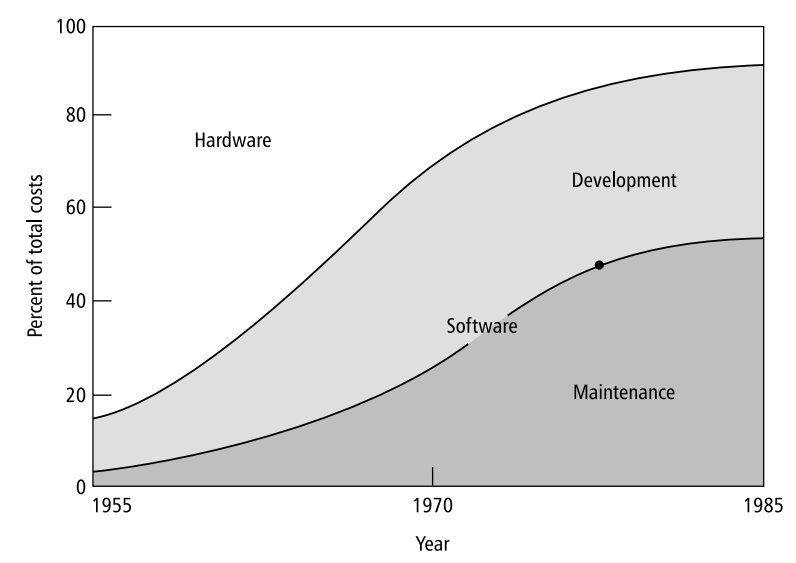
\includegraphics[scale=2.2]{images/chapter2/software_engineering/hardware_software_costs.png}
    \caption{Σχετική κατανομή κόστους υλικού/λογισμικού (\textsl{Πηγή: \cite{hardware_software_costs}}) }
    \label{fig:hardware_software_costs}
\end{figure}

Η διαφορά κόστους έγκειται στο γεγονός ότι τα σύγχρονα προγράμματα λογισμικού είναι μεγάλα και περίπλοκα, απαιτώντας ομάδες υψηλής εξειδίκευσης, δεν έχουν περιορισμούς (δηλαδή έχουν περισσότερους βαθμούς ελευθερίας) και τέλος επειδή υφίσταται συνεχόμενες αλλαγές. Μάλιστα, στη διάρκεια ζωής του λογισμικού οι αλλαγές αυτές ενδέχεται να εισάγουν σφάλματα, αυξάνοντας τον κίνδυνο αποτυχίας του συστήματος, όπως φαίνεται στο Σχήμα \ref{fig:software_failure_rate}. Επιπλέον, σε αντίθεση με την αποτυχία του υλικού, όπου αντιμετωπίζεται με αντικατάσταση του χαλασμένου μέρους, η αποτυχία του λογισμικού έγκειται σε σφάλμα σχεδιασμού, καθιστώντας τη συντήρηση του σημαντικά πιο περίπλοκη και ακριβή διαδικασία.

\begin{figure}[h]
    \centering
    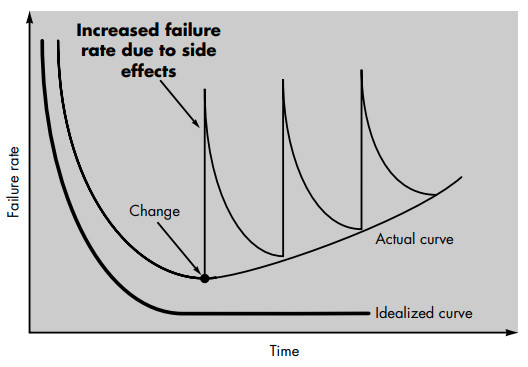
\includegraphics[scale=2.2]{images/chapter2/software_engineering/software_failure_rate.jpg}
    \caption{Καμπύλη αποτυχίας για το λογισμικό}
    \label{fig:software_failure_rate}
\end{figure}

Εντούτοις, η αυξανόμενη εξάρτηση των καθημερινών δραστηριοτήτων από περίπλοκα συστήματα λογισμικού απαιτεί την εύρωστη και αλάνθαστη λειτουργία τους καθ' όλη τη διάρκεια ζωής του λογισμικού, το οποίο όμως αλλάζει συνεχώς αυξάνοντας τον κίνδυνο αποτυχίας του. Τοιουτοτρόπως, για την μείωση του ρίσκου αποτυχίας και την απλούστευση της ανάπτυξης και συντήρησης υψηλής ποιότητας έργων λογισμικού, έπρεπε να τυποποιηθούν οι μέθοδοι και διαδικασίες που διέπουν ολόκληρο τον κύκλο ζωής του. Αυτές οι μεθοδολογίες εμπεριέχονται και αναλύονται από την επιστήμη της τεχνολογίας λογισμικού.

\subsection{Τεχνολογία Λογισμικού}

Η τεχνολογία λογισμικού είναι η συστηματική, πειθαρχημένη και μετρήσιμη προσέγγιση με σκοπό την ανάπτυξη, λειτουργία και συντήρηση υψηλής ποιότητας έργων λογισμικού. Οι διαδικασίες της τεχνολογίας λογισμικού παρέχουν ένα ευρύτερο πλαίσιο, μέσα στο οποίο εφαρμόζονται οι τεχνικές μέθοδοι, παράγονται προϊόντα δουλειάς (μοντέλα, έγγραφα, δεδομένα, αναφορές κ.α.), εξακριβώνονται σημεία σταθμοί, εξασφαλίζεται η ποιότητα και γίνεται κατάλληλη διαχείριση των αλλαγών των απαιτήσεων.

Οι μέθοδοι της τεχνολογίας λογισμικού είναι το τεχνικό εγχειρίδιο για την ανάπτυξη λογισμικού. Οι μέθοδοι εγκολπώνουν ένα ευρύ σύνολο λειτουργιών συμπεριλαμβανομένων την ανάλυση απαιτήσεων, σχεδιασμού, δημιουργία προγράμματος, δοκιμής και υποστήριξης. Οι μέθοδοι της τεχνολογίας λογισμικού βασίζονται σε βασικές αρχές και πρακτικές που διέπουν κάθε τομέα της τεχνολογίας και περιλαμβάνουν δραστηριότητες μοντελοποίησης και άλλες περιγραφικές τεχνικές.

\subsubsection{Πλαίσιο διαδικασίας}

Το πλαίσιο διαδικασίας της τεχνολογίας λογισμικού απαρτίζεται από δραστηριότητες που είναι κοινές για οποιοδήποτε έργο λογισμικού ανεξάρτητα από το μέγεθος και την περιπλοκότητα του. Ένα γενικό πλαίσιο διαδικασίας περιλαμβάνει πέντε κύριες δραστηριότητες \cite{software_engineering_practiotioner_approach}:

\begin{itemize}
    \item \textbf{Επικοινωνία} (Communication): Πριν την έναρξη οποιασδήποτε τεχνικής εργασίας, είναι άκρως σημαντική η επικοινωνία και συνεργασία με τον πελάτη (και άλλα ενδιαφερόμενα μέλη). Η πρόθεση είναι η κατανόηση των στόχων των ενδιαφερόμενων μελών για το έργο λογισμικού και η συλλογή απαιτήσεων, βοηθώντας τον καθορισμό των λειτουργιών και των χαρακτηριστικών του λογισμικού.
    \item \textbf{Προγραμματισμός} (Planning): Ένα έργο λογισμικού είναι ένα περίπλοκο ταξίδι και η διαδικασία του προγραμματισμού είναι ο χάρτης ο οποίος οδηγεί την ομάδα ανάπτυξης. Το σχέδιο του έργου αποσαφηνίζει την απαιτούμενη δουλειά, περιγράφοντας τις τεχνικές εργασίες προς διεκπεραίωση, τα πιθανά ρίσκα, τους απαιτούμενους πόρους, τα προϊόντα προς παραγωγή και το πρόγραμμα εργασίας. 
    \item \textbf{Μοντελοποίηση} (Modelling): Δημιουργούνται μοντέλα ώστε να γίνει εφικτή η καλύτερη κατανόηση των απαιτήσεων του λογισμικού και του σχεδιασμού ο οποίος δύναται να ικανοποιήσει αυτές τις απαιτήσεις. Γίνεται εμφανής η αρχιτεκτονική μορφή του έργου, ο τρόπος αλληλεξάρτησης των μεμονωμένων μερών και πολλά άλλα χαρακτηριστικά, στη προσπάθεια κατανόησης του προβλήματος και του τρόπου επίλυσης του.
    \item \textbf{Κατασκευή} (Construction): Η δραστηριότητα αυτή περιλαμβάνει την υλοποίηση του έργου παράγοντας κώδικα (είτε με χειροκίνητο ή αυτόματο τρόπο) και τον έλεγχο του κώδικα για την ανίχνευση σφαλμάτων. 
    \item \textbf{Εγκατάσταση} (Deployment): Το λογισμικό ως ολόκληρη οντότητα ή σε επιμέρους διαδοχικά στάδια παραδίνεται στον πελάτη ο οποίος αξιολογεί το παραδοθέν προϊόν και παρέχει ανατροφοδότηση.
\end{itemize}

Σε πολλά έργα λογισμικού, οι δραστηριότητες πλαισίου εφαρμόζονται επαναληπτικά καθώς αναπτύσσεται το έργο. Κάθε επανάληψη παράγει μία επαύξηση του λογισμικού η οποία θέτει στην διάθεση των ενδιαφερόμενων μελών ένα υποσύνολο των τελικών χαρακτηριστικών και λειτουργιών του λογισμικού. Τοιουτοτρόπως, το λογισμικό ολοκληρώνεται σταδιακά με το πέρας κάθε επανάληψης. 

\subsection{Ροές διαδικασίας Τεχνολογίας Λογισμικού}

Μία διαδικασία ορίζεται ως το άθροισμα των δραστηριοτήτων, ενεργειών και εργασιών που πρέπει να διεκπεραιωθούν με σκοπό την παραγωγή ενός προϊόντος εργασίας. Όπως αναφέρθηκε παραπάνω, το γενικό πλαίσιο διαδικασίας του λογισμικού αποτελείται από πέντε δραστηριότητες σε συνδυασμό με άλλες ενέργειες - όπως παρακολούθηση και έλεγχος έργου, εκτίμηση και διαχείριση ρίσκου, διασφάλιση ποιότητας, ρύθμιση παραμέτρων κ.α. - που εφαρμόζονται καθ' όλη την διαδικασία.

Η ροή διαδικασίας περιγράφει τον τρόπο με τον οποίο οι δραστηριότητες πλαισίου, οι ενέργειες και οι εργασίες εντός κάθε δραστηριότητας οργανώνονται σε σχέση με την αλληλουχία τους και τον χρόνο όπως φαίνεται στο Σχήμα \ref{fig:software_process_flow}.

\begin{figure}[h!]
    \begin{subfigure}{\linewidth}
        \centering
        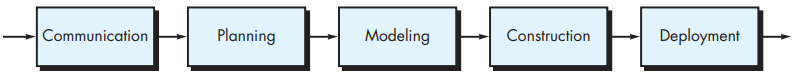
\includegraphics[scale=0.5]{images/chapter2/software_engineering/linear_process_flow.png}
        \caption{Γραμμική ροή}
        \label{subfig:linear_flow}
    \end{subfigure}\par\medskip
    \begin{subfigure}{\linewidth}
        \centering
        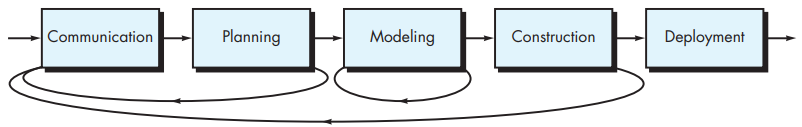
\includegraphics[scale=0.5]{images/chapter2/software_engineering/iterative_process_flow.png}
        \caption{Επαναληπτική ροή}
        \label{subfig:iterative_flow}
    \end{subfigure}\par\medskip
    \begin{subfigure}{\linewidth}
        \centering
        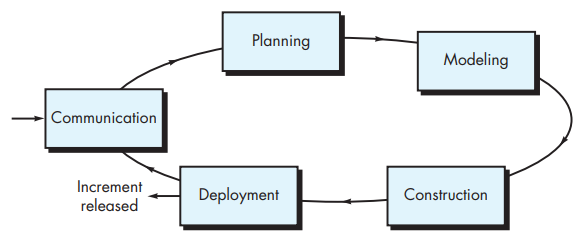
\includegraphics[width=0.7\linewidth]{images/chapter2/software_engineering/evolutionery_process_flow.png}
        \caption{Εξελικτική ροή}
        \label{subfig:evolutionery_flow}
    \end{subfigure}
    \begin{subfigure}{\linewidth}
        \centering
        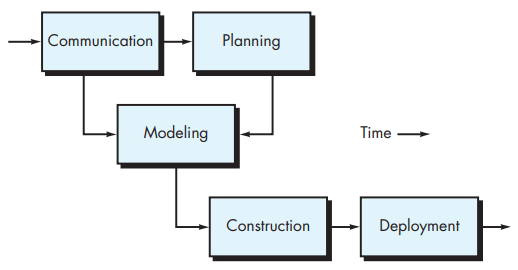
\includegraphics[width=0.7\linewidth]{images/chapter2/software_engineering/parallel_process_flow.png}
        \caption{Παράλληλή ροή}
        \label{subfig:parallel_flow}
    \end{subfigure}
    \caption{Ροές διαδικασίας λογισμικού}
    \label{fig:software_process_flow}
\end{figure}

H γραμμική ροή εκτελεί τις δραστηριότητες διαδοχικά, ξεκινώντας την κάθε δραστηριότητα με το πέρας της προηγούμενης (\ref{subfig:linear_flow}). Η επαναληπτική ροή επαναλαμβάνει μία ή περισσότερες δραστηριότητες πριν προχωρήσει στην επόμενη (\ref{subfig:iterative_flow}).H εξελικτική ροή εκτελεί τις δραστηριότητες κυκλικά. Στο πέρας της διεκπεραίωσης των δραστηριοτήτων παράγεται σταδιακά η εφαρμογή ολοένα και πιο ολοκληρωμένη (\ref{subfig:evolutionery_flow}). Η παράλληλη ροή (\ref{subfig:parallel_flow}) εκτελεί μία ή περισσότερες δραστηριότητες παράλληλα με άλλες δραστηριότητες (για παράδειγμα η μοντελοποίηση μιας πτυχής του λογισμικού μπορεί να γίνεται ταυτόχρονα με την κατασκευή μιας άλλης πτυχής του).

\subsection{Μοντέλα ανάπτυξης λογισμικού}

\subsubsection{Μοντέλο Καταρράκτη}

Το μοντέλο ανάπτυξης \textsl{καταρράκτη} ακολουθεί την γραμμική ροή, δηλαδή οι δραστηριότητες από την \textsl{επικοινωνία} μέχρι την \textsl{εγκατάσταση} διεκπεραιώνονται διαδοχικά. Το μοντέλο αυτό επιλέγεται όταν οι απαιτήσεις του λογισμικού είναι ξεκάθαρα ορισμένες και επαρκώς σταθερές.

Το μοντέλο \textsl{καταρράκτη} είναι το παλαιότερο μοντέλο της τεχνολογίας λογισμικού. Εντούτοις, με την εξέλιξη της τεχνολογίας και των απαιτήσεων έχει παρουσιάσει πληθώρα προβλημάτων.

\begin{itemize}
  \item Τα έργα λογισμικού σπάνια ακολουθούν την προτεινόμενη γραμμική ροή. Τοιουτοτρόπως, οι αλλαγές δεν είναι εύκολα διαχειρίσιμες και μπορεί να προκαλέσουν σύγχυση. 
  \item Συνήθως είναι δύσκολο για τον πελάτη να καθορίσει όλες τις απαιτήσεις αναλυτικά. Το μοντέλο \textsl{καταρράκτη} όμως το απαιτεί και έτσι δεν μπορεί να διαχειριστεί την αβεβαιότητα που έγκειται στην έναρξη οποιουδήποτε έργου λογισμικού.
  \item Μία λειτουργική έκδοση του λογισμικού γίνεται διαθέσιμη αρκετά αργά στην διάρκεια ζωής του έργου. Έτσι, από την μία ο πελάτης πρέπει να είναι υπομονετικός και από την άλλη μία αστοχία σχεδιασμού που θα ανιχνευτεί κατά την αξιολόγηση της λειτουργικής έκδοσης μπορεί να είναι καταστροφική.
\end{itemize}

\subsubsection{Αυξητικό Μοντέλο}

Το \textsl{αυξητικό} μοντέλο συνδυάζει την γραμμική και την παράλληλη ροή διαδικασιών. Όπως φαίνεται στο Σχήμα \ref{fig:incremental_process_model}, το αυξητικό μοντέλο χωρίζει τις λειτουργίες και τα χαρακτηριστικά του λογισμικού σε μικρές επαυξήσεις και για κάθε επαύξηση διεκπεραιώνει γραμμικά τις δραστηριότητες, στο πέρας των οποίων παραδίδεται η λειτουργία του λογισμικού.

\begin{figure}[h]
    \centering
    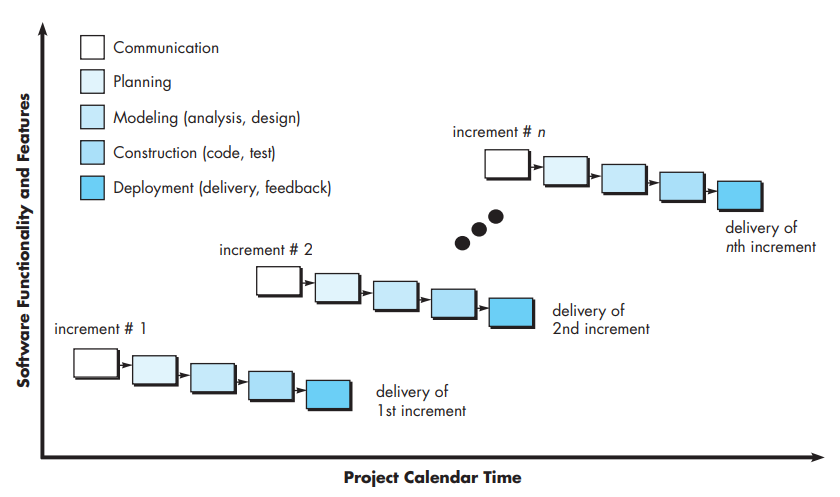
\includegraphics[scale=2]{images/chapter2/software_engineering/incremental_process_model.png}
    \caption{Αυξητικό Μοντέλο}
    \label{fig:incremental_process_model}
\end{figure}

Οι πρώτες επαυξήσεις υλοποιούν τις κυριότερες λειτουργίες του λογισμικού, ικανοποιώντας τις αρχικές απαιτήσεις. Το προϊόν παραδίδεται στον πελάτη ή υπόκειται σε λεπτομερή αξιολόγηση. Τοιουτοτρόπως, αναπτύσσεται ένα σχέδιο για τις επόμενες επαυξήσεις. Το σχέδιο αφορά τις αλλαγές του κύριου προϊόντος, με σκοπό την καλύτερη ικανοποίηση των απαιτήσεων του πελάτη, και την ανάπτυξη επιπλέον χαρακτηριστικών και λειτουργιών. Η διαδικασία επαναλαμβάνεται μετά από την παράδοση κάθε επαύξησης έως ότου ολοκληρωθεί το λογισμικό.

Το αυξητικό μοντέλο είναι ιδανικό όταν υπάρχουν κάποιες πλήρης και καλά καθορισμένες απαιτήσεις με χαλαρά συζευγμένα μέρη. Έτσι, οι αρχικές επαυξήσεις μπορούν να προγραμματιστούν και να παραλληλοποιηθούν επαρκώς.

\subsubsection{Σπειροειδές Μοντέλο}

Το \textsl{σπειροειδές} μοντέλο είναι ένα εξελικτικό μοντέλο με κύριο γνώμονα το ρίσκο. Όπως και στο \textsl{αυξητικό} μοντέλο το λογισμικό παραδίδεται σε επαναλήψεις, όμως σε αντίθεση με αυτό τα βήματα δεν είναι δραστηριότητες αλλά φάσεις, με σκοπό την αντιμετώπιση του προβλήματος με το μεγαλύτερο ρίσκο να προκαλέσει αποτυχία.

\begin{figure}[h]
    \centering
    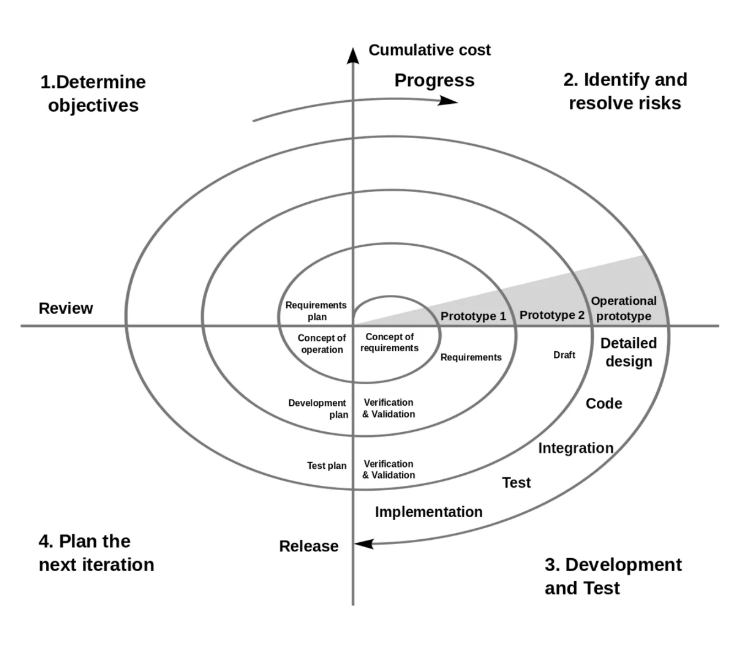
\includegraphics[scale=2]{images/chapter2/software_engineering/spiral_process_model.png}
    \caption{Σπειροειδές Μοντέλο}
    \label{fig:spiral_process_model}
\end{figure}

Όπως φαίνεται στο Σχήμα \ref{fig:spiral_process_model}, οι φάσεις σε κάθε επανάληψη είναι:
\begin{enumerate}
    \item Εξακρίβωση του προβλήματος με το μεγαλύτερο ρίσκο, καθορισμός των στόχων και των εναλλακτικών λύσεων.
    \item Αξιολόγηση και σχεδιασμός των πιθανών λύσεων και προσδιορισμός των ρίσκων.
    \item Ανάπτυξη μίας λύσης, επιβεβαίωση καταλληλότητας και δοκιμή της
    \item Προετοιμασία για την επόμενη επανάληψη με βάση την ανατροφοδότηση από την παραδοθείσα επαύξηση.
\end{enumerate}

Το σπειροειδής μοντέλο μπορεί να διαχειριστεί την αβεβαιότητα εξαιρετικά καλά. Έτσι, είναι ιδανικό για έργα λογισμικού με ασαφή απαιτήσεις και για έργα που βρίσκονται στην έρευνα και ανάπτυξη.

\subsubsection{Ευέλικτο Μοντέλο}
Στη σύγχρονη πραγματικότητα, η εργασία στην παραγωγή λογισμικού έχει ταχύς ρυθμούς και είναι υποκείμενο σε συνεχή ροή αλλαγών (χαρακτηριστικών, λειτουργιών και πληροφοριακού περιεχόμενου). Έτσι, το \textsl{ευέλικτο} μοντέλο αποτελεί μία λογική εναλλακτική στις παραδοσιακές μεθόδους της τεχνολογίας λογισμικού. 

Το μοντέλο ενθαρρύνει συνεχόμενες επαναλήψεις από ανάπτυξη και δοκιμή των λειτουργιών. Σε κάθε επανάληψη παράγεται μία επαύξηση του λογισμικού αποτελούμενη από ένα μικρό σύνολο από λειτουργίες πλήρως ολοκληρωμένες. Επίσης, η κάθε επανάληψη είναι σχεδιασμένη ώστε να είναι μικρή, διαχειρίσιμη και ολοκληρώσιμη σε λίγες εβδομάδες. Συμπεριλαμβάνει των πελάτη στην διαδικασία της ανάπτυξης και ελαχιστοποιεί τα έγγραφα χρησιμοποιώντας ανεπίσημη επικοινωνία.

Το ευέλικτο μοντέλο αν και αποτελεί ρεαλιστική προσέγγιση στην ανάπτυξη λογισμικού, βρίσκεται σε μειονεκτική θέση όταν το λογισμικό είναι σύνθετο. Επίσης, αδυνατεί να διαχειριστεί τις μεταβιβάσεις λόγω των λίγων εγγράφων, αλλά από την άλλη μπορεί να διαχειριστεί τις μεταβαλλόμενες απαιτήσεις.

Οι πιο συνηθισμένες ευέλικτες μεθοδολογίες είναι:

\begin{itemize}
    \item \textbf{Scrum}: Αποτελείται από επαναλήψεις που λέγονται sprints. Κάθε sprint διαρκεί 2 με 4 εβδομάδες και πριν την έναρξη του γίνεται προγραμματισμός. Αφού οριστούν οι δραστηριότητες και οι εργασίες για το sprint δεν μεταβάλλονται κατά την διάρκειά του.
    \item \textbf{Extreme Programming (XP)}: Σε αυτό το μοντέλο η επανάληψη διαρκεί 1 με 2 εβδομάδες. Χαρακτηριστικά αυτού του μοντέλου είναι ο προγραμματισμός σε ζεύγη, η ανάπτυξη οδηγούμενη από έλεγχο (test-driven development), ο αυτοματοποιημένος έλεγχος, η απλή σχεδίασμη λογισμικού και τέλος οι μικρές εκδόσεις με συνεχόμενη ενσωμάτωση στο σύστημα.
    \item \textbf{Kanban}: Το μοντέλο Kanban επικεντρώνεται στην οπτικοποίηση, και αν υπάρχουν επαναλήψεις είναι πολύ μικρές. Στο πίνακα Kanban παριστάνονται όλες οι δραστηριότητες και εργασίες του έργου, συνοδευόμενες από τα υπεύθυνα άτομα για την διεκπεραίωσή τους και την πρόοδό τους.
\end{itemize}


\subsection{Σχεδιαστικά Πρότυπα}
Πράγματι, οι σύγχρονες επιχειρήσεις στρέφονται ολοένα και περισσότερο προς τα \textsl{ευέλικτα μοντέλα} ανάπτυξης λογισμικού για την διαχείριση των μεταβαλλόμενων απαιτήσεων. Εντούτοις, τα \textsl{ευέλικτα μοντέλα} απαιτούν απλό σχεδιασμό του λογισμικού έτσι ώστε να μπορούν να επεκταθούν. Προς επίτευξη αυτού του σκοπού, καθίσταται επιτακτική η ανάγκη αναζήτησης και εφαρμογής σχεδιαστικών προτύπων.

Ο σκοπός των σχεδιαστικών προτύπων είναι να παρέχουν γενικές λύσεις σε συνηθισμένα προβλήματα του σχεδιασμού λογισμικού. Τυποποιώντας επίσημα τις λύσεις και τις σχέσεις μεταξύ τους καθίσταται